\section{块坐标下降（BCD）}
\label{sec:block-bcd}

上一节把变量分成了块。接下来要弄清：每次选一块、固定其余变量并改善完整目标，这个过程应当怎样组织？

\term{块坐标下降}（block coordinate descent，BCD）把一次迭代拆成两个环节：选块决定这一步动哪一块，块内更新决定这一块怎样动。两个环节可以自由搭配。本节先固定块内更新为“精确求解条件子问题”，集中比较循环、随机、贪心三种选块方式；第~\ref{sec:block-local}节以后再替换块内更新。

这些选块规则也能用于后面的梯度、邻近或模型更新，但搭配之后的下降和收敛保证要重新核对，不能直接搬用。

\subsection{精确块更新}
\label{sec:block-exact}

\paragraph{更新规则}
设可行集是乘积形式~\eqref{eq:block-product-set}，当前点为$\bm{x}^{(t)}$，选中块$J$。精确块更新在块$J$的允许集合上最小化条件函数，其他块不动：
\begin{equation}
 \bm{x}_J^{(t+1)}\in\argmin_{\bm{z}\in\bm{C}_J}\varphi_J(\bm{z};\bm{x}^{(t)}),\qquad
 \bm{x}_{i}^{(t+1)}=\bm{x}_{i}^{(t)}\ \ (i\notin J).
 \label{eq:block-exact}
\end{equation}
这里的“$\in$”提醒我们最小点可能不止一个。

\paragraph{完整目标不增}
这个规则带来的进展来自一个简单的比较：当前的$\bm{x}_J^{(t)}$本身就是子问题的一个候选，最优解不会比它差。其他块又没有改变，所以条件函数的值就是完整目标的值。

\begin{lemma}[精确块更新的单调性]
\label{lem:block-exact-descent}
设可行集有乘积结构~\eqref{eq:block-product-set}，$\bm{x}^{(t)}\in\bm{C}$，且条件子问题的最小点存在。按式~\eqref{eq:block-exact}更新后$\bm{x}^{(t+1)}\in\bm{C}$，并且
\begin{equation}
 f(\bm{x}^{(t+1)})\leq f(\bm{x}^{(t)}).
 \label{eq:block-exact-monotone}
\end{equation}
\end{lemma}

\begin{proof}
其他块未变，块$J$落在$\bm{C}_J$内，乘积结构保证新点可行。$\bm{x}_J^{(t)}\in\bm{C}_J$是条件子问题的可行点，最小点的函数值不超过它的函数值，于是
\[
 \varphi_J(\bm{x}_J^{(t+1)};\bm{x}^{(t)})\leq\varphi_J(\bm{x}_J^{(t)};\bm{x}^{(t)}).
\]
由定义~\eqref{eq:block-conditional}，左边等于$f(\bm{x}^{(t+1)})$，右边等于$f(\bm{x}^{(t)})$。
\end{proof}

\paragraph{两件要先核对的事}
引理假定最小点存在，这一条并非总成立。取$f(x_1,x_2)=e^{x_1}+x_2^2$，固定$x_2$后，条件函数沿$x_1\to-\infty$递减而取不到最小值，更新规则根本没有定义。使用精确块更新前，要用条件函数的紧下水平集之类的条件确认最小点存在。

最小点也可能不唯一。取$\tfrac12(uv-1)^2$，固定$v=0$时，条件函数恒等于$\tfrac12$，每个$u$都是最小点。这时算法必须事先规定怎样选，常见的规则有“当前值已是最小点就不动”或“取离当前点最近的最小点”。没有这样的规则，迭代序列就没有确定的含义，第~\ref{sec:block-convergence}小节会看到，解的选择还影响收敛结论。

\paragraph{二次目标的块解}
对二次目标，条件子问题有显式解。设
\[
 f(\bm{x})=\frac12\bm{x}^\top\bm{Q}\bm{x}-\bm{b}^\top\bm{x},
\]
其中$\bm{Q}$对称，块$J$的主子矩阵$\bm{Q}_{J,J}$正定，$\bar{J}$是$J$的补集。令偏梯度为零，
\[
 \bm{Q}_{J,J}\bm{x}_J+\bm{Q}_{J,\bar{J}}\bm{x}_{\bar{J}}-\bm{b}_J=\bm{0},
\]
解出
\begin{equation}
 \bm{x}_J^{+}=\bm{Q}_{J,J}^{-1}\bigl(\bm{b}_J-\bm{Q}_{J,\bar{J}}\bm{x}_{\bar{J}}\bigr).
 \label{eq:block-quadratic-solve}
\end{equation}

在式~\eqref{eq:block-example}中更新$x_1$。固定$x_2=4$，条件函数是
\[
 \varphi(z)=z^2+4z+16,
\]
令导数$2z+4=0$，得到
\[
 z=-2,\qquad \varphi(-2)=12 .
\]

条件子问题已经精确解出，$x_1$在固定$x_2=4$时不可能更好了。但点$(-2,4)$不是原问题的解，它的目标值是$12$，而$f^\star=0$；它的梯度也不为零：
\[
 \nabla f(-2,4)=(0,\,6).
\]
第一个分量为零，说明$x_1$这一块确实调好了；第二个分量不为零，说明$x_2$还没有。图~\ref{fig:block-exact-slice}把这两件事画在一起。

\begin{BookInlineFigure}
  \centering
  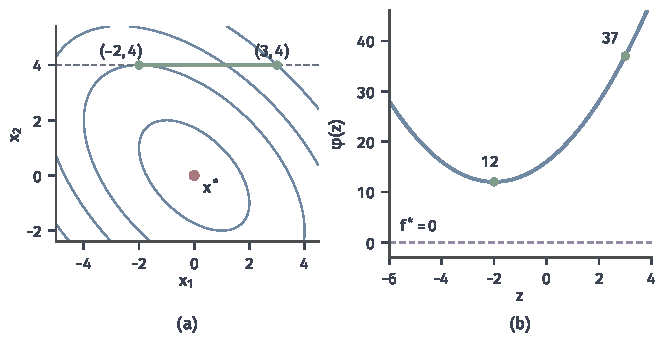
\includegraphics[width=112mm]{figures/05-optimization/04-block-optimization/matplotlib/block-exact-slice/figure.pdf}
  \caption{精确解条件子问题与解出整个问题的差别。(a)固定$x_2=4$（灰色虚线），在这条直线上从$(3,4)$移到条件最小点$(-2,4)$，该点处等高线与虚线相切，但离红色的最优解还远。(b)沿虚线的条件函数$\varphi(z)=z^2+4z+16$，绿点的值从$37$降到$12$；紫色虚线是完整问题的最优值$0$。}
  \label{fig:block-exact-slice}
\end{BookInlineFigure}

\subsection{循环块坐标下降（Cyclic BCD）}
\label{sec:block-cyclic}

\paragraph{主要思想}
最朴素的选块方式是按固定顺序轮流，这就是\term{循环块坐标下降}（cyclic block coordinate descent）。依次把$J_1,\ldots,J_B$各更新一次称为一\term{轮}（epoch）。后面的块读取的是本轮已经更新的新值，这一点很关键：刚得到的信息立刻被用上。

对二次目标，单坐标的循环更新就是线性方程组的Gauss--Seidel迭代，其收敛条件和误差传播的矩阵形式，可参考\BookChapterRef{chap:stationary-iterations}{卷二第14章“定常迭代法”}。这里我们关心的是耦合怎样决定速度。

把式~\eqref{eq:block-example}中的交叉项系数换成参数$c$，$\lvert c\rvert<2$，考虑
\begin{equation}
 f_c(\bm{x})=x_1^2+cx_1x_2+x_2^2 .
 \label{eq:block-coupling-family}
\end{equation}
令$\partial_1f_c=2x_1+cx_2=0$，$\partial_2f_c=cx_1+2x_2=0$，得到两条更新规则
\begin{equation}
 x_1\leftarrow-\frac{c}{2}x_2,\qquad x_2\leftarrow-\frac{c}{2}x_1 .
 \label{eq:block-cyclic-update}
\end{equation}

第一步之后，$x_1=-\tfrac{c}{2}x_2$总是成立，把它代入第二条规则，$x_2$的新值是旧值的$(c/2)^2$倍。所以从第二轮起，每一轮
\begin{equation}
 x_2^{\mathrm{new}}=\Bigl(\frac{c}{2}\Bigr)^{2}x_2^{\mathrm{old}} .
 \label{eq:block-cyclic-factor}
\end{equation}
$c=0$时没有耦合，一轮就到最优解；$c$越接近$2$，等高线越扁越斜，收缩越慢。

\needspace{6\baselineskip}
\paragraph{变量}
\begin{itemize}
 \item $\bm{x}^{(t)}$：第$t$轮结束时的点，在原处逐块覆盖。
 \item $J_1,\ldots,J_B$：固定的块顺序。例中$B=2$，$J_1=\{1\}$，$J_2=\{2\}$。
 \item $\varepsilon$：完整梯度范数的容差。
\end{itemize}

\paragraph{初始化}
选定可行的起点和块顺序，令$t=0$。例中用式~\eqref{eq:block-example}，$c=1$，容差$\varepsilon=10^{-3}$，起点是
\[
 \bm{x}^{(0)}=(3,4),\qquad f(\bm{x}^{(0)})=37 .
\]

\needspace{6\baselineskip}
\paragraph{每轮更新}
在第$t$轮中，对$k=1,\ldots,B$依次执行：
\begin{enumerate}
 \item \textbf{读取新值。}固定其他块的最新取值，形成块$J_k$的条件子问题。
 \item \textbf{精确求解。}按式~\eqref{eq:block-exact}更新块$J_k$。例中第一轮由式~\eqref{eq:block-cyclic-update}，先用$x_2=4$更新$x_1$，再用新的$x_1$更新$x_2$：
 \[
  x_1=-2,\qquad x_2=1 .
 \]
 两次更新后的目标值依次是$12$和$3$。

 例中第二轮读到$x_2=1$，然后读到新的$x_1$：
 \[
  x_1=-\tfrac12,\qquad x_2=\tfrac14 .
 \]
 目标值依次是$\tfrac34$和$\tfrac{3}{16}$。

 例中第三轮得到
 \[
  x_1=-\tfrac18,\qquad x_2=\tfrac{1}{16},
 \]
 目标值依次是$\tfrac{3}{64}$和$\tfrac{3}{256}$。
 \item \textbf{检查停止。}一轮结束后计算$\lVert\nabla f(\bm{x}^{(t+1)})\rVert_2$，不超过$\varepsilon$就停止，否则令$t\leftarrow t+1$。例中第$t$轮结束时
 \[
  \nabla f(\bm{x}^{(t)})=\bigl(-3\cdot4^{1-t},\ 0\bigr).
 \]
\end{enumerate}

规律很清楚：第一步之后，每做一次坐标更新，目标值乘以$\tfrac14$。第$t$轮结束时
\[
 \bm{x}^{(t)}=\bigl(-2\cdot4^{1-t},\ 4^{1-t}\bigr),\qquad
 f(\bm{x}^{(t)})=3\cdot16^{1-t}.
\]
梯度范数不超过$10^{-3}$要求$3\cdot4^{1-t}\leq10^{-3}$，即$t\geq7$。最终得到
\[
 \bm{x}^{(7)}=\bigl(-4.88\times10^{-4},\ 2.44\times10^{-4}\bigr).
\]

\paragraph{耦合与顺序的影响}
图~\ref{fig:block-cyclic-staircase}画出了两种耦合下的阶梯路径。(a)中$c=1$，先更新$x_1$的路径向左上转折，先更新$x_2$的路径向右下转折：顺序改变路径，但两条路径都按因子$\tfrac14$收缩。(b)中$c=1.8$，路径沿狭长的谷底爬行，每一阶都很短，每轮收缩因子变成$0.81$。

\begin{BookInlineFigure}
  \centering
  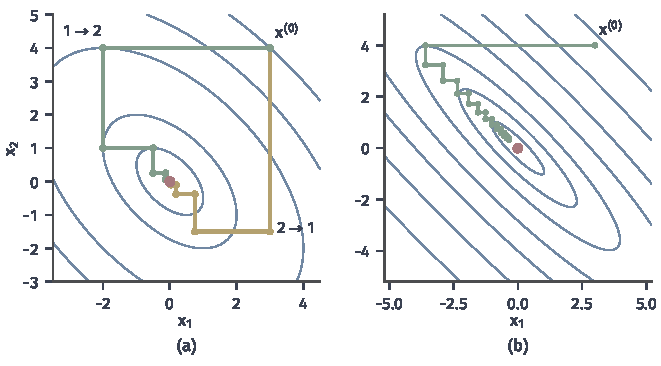
\includegraphics[width=112mm]{figures/05-optimization/04-block-optimization/matplotlib/block-cyclic-staircase/figure.pdf}
  \caption{循环坐标下降的阶梯路径，从$(3,4)$出发。(a)$c=1$，绿色先更新$x_1$，黄色先更新$x_2$，各画三轮，都按式~\eqref{eq:block-cyclic-factor}的因子$\tfrac14$收缩。(b)$c=1.8$，绿色路径画十二轮，变量耦合越强，每一阶越短。}
  \label{fig:block-cyclic-staircase}
\end{BookInlineFigure}

阶梯形状的来源是：每次只能沿坐标轴走，而谷底方向是斜的。这好比在只能走东西、南北方向的棋盘式街道上，要朝东北方向下山，只能东一段、北一段地拼出来，而且每一段都不能走得太远，否则就偏离了谷底。变量的耦合就是这条斜谷的走向，耦合越强，能走的每一段越短。

\paragraph{固定循环与每轮打乱}
二维时顺序只影响第一步，维数高了影响会大得多。实践中常在每轮开始时重新打乱顺序，这称为随机重排。它与固定循环的差别在于顺序每轮不同，与下一小节的独立随机选块的差别在于一轮内每块恰好出现一次。

后一个差别在分析中很要紧。一轮内已经选过的块不会再被选到，所以“这一步选到块$J$的概率”依赖于本轮前面选过什么，不再是与历史无关的固定值。下一小节取条件期望的论证用不上，每轮打乱的收敛分析要另外处理。

图~\ref{fig:block-order-compare}是一个数值实例。这个目标的各个变量两两等强度耦合，起点随机，固定循环明显慢于另外两种规则，每轮打乱和独立随机几乎一样。这只是一个具体问题上的观察，不是普遍定理；在另外的问题上，固定循环可以和随机规则一样快。

\begin{BookInlineFigure}
  \centering
  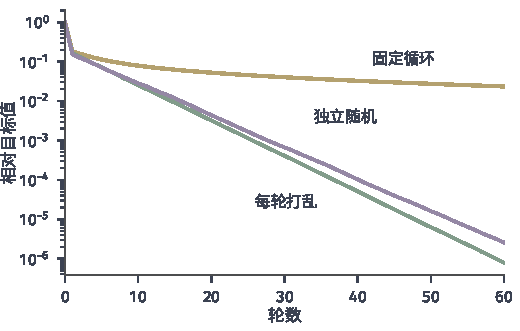
\includegraphics[width=88mm]{figures/05-optimization/04-block-optimization/matplotlib/block-order-compare/figure.pdf}
  \caption{三种更新顺序在同一目标上的比较。目标为$\tfrac12\bm{x}^\top\bm{Q}\bm{x}$，$\bm{Q}=0.1\,\bm{I}+0.9\,\bm{1}\bm{1}^\top$，$n=30$，单坐标精确更新，纵轴为目标值与起点目标值之比。黄线是固定循环，绿线是每轮打乱，紫线是独立随机（每轮$n$次更新），后两者是$30$次重复的几何平均。}
  \label{fig:block-order-compare}
\end{BookInlineFigure}

\subsection{随机块坐标下降（RBCD）}
\label{sec:block-random}

\paragraph{主要思想}
循环规则的路径取决于顺序，分析也依赖整轮的累积效应。如果每步独立地抽一块，就可以用平均值来分析单步进展，这是\term{随机块坐标下降}（randomized block coordinate descent，RBCD）的出发点。

设第$t$步与历史独立地以固定概率$p_J>0$抽取块$J$，$\sum_Jp_J=1$。记块$J$精确更新带来的真实下降量为$\Delta_J(\bm{x})=f(\bm{x})-f(\bm{x}^{+J})$，其中$\bm{x}^{+J}$是只更新块$J$得到的点。已知当前点$\bm{x}^{(t)}$时，新点的目标值是随机的，它的条件期望是各种可能结果的加权平均：
\begin{equation}
 \mathbb{E}\bigl[f(\bm{x}^{(t+1)})\mid\bm{x}^{(t)}\bigr]
 =f(\bm{x}^{(t)})-\sum_{J}p_J\,\Delta_J(\bm{x}^{(t)}).
 \label{eq:block-random-expectation}
\end{equation}
这里只用到离散情形的加权平均，条件期望的一般定义可参考\BookChapterRef{chap:conditional-expectation}{卷七第4章“条件期望与条件分布”}。

式~\eqref{eq:block-random-expectation}说明，随机规则的平均进展就是各块进展的加权平均，所以只要每块都有保底的进展，平均也有。

\paragraph{单步平均的计算}
对单坐标精确更新的二次目标，真实下降量可以写出来。条件函数是开口系数为$Q_{j,j}/2$的抛物线，当前斜率是$\partial_jf$，最小化后下降
\begin{equation}
 \Delta_j(\bm{x})=\frac{(\partial_jf(\bm{x}))^2}{2Q_{j,j}} .
 \label{eq:block-coordinate-decrease}
\end{equation}

在起点$(3,4)$，偏导数和两个下降量是
\[
 \partial_1f=10,\qquad \partial_2f=11,\qquad \Delta_1=25,\qquad \Delta_2=\frac{121}{4}=30.25 .
\]
均匀抽取时，平均下降量是
\[
 \frac12(25+30.25)=27.625,
\]
平均目标值是$37-27.625=9.375$。图~\ref{fig:block-random-average}把两个可能的结果和平均值放在一起。

\begin{BookInlineFigure}
  \centering
  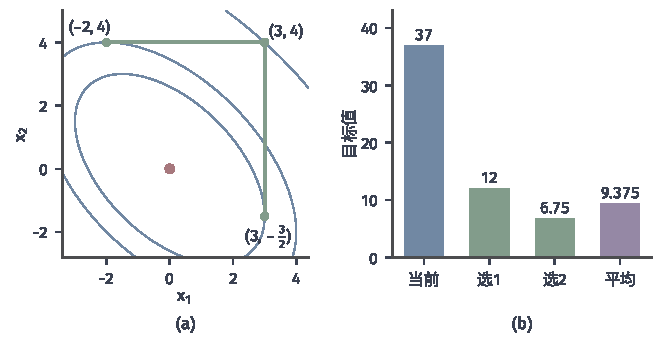
\includegraphics[width=112mm]{figures/05-optimization/04-block-optimization/matplotlib/block-random-average/figure.pdf}
  \caption{随机选块的一步。(a)从$(3,4)$出发，抽到$x_1$走到$(-2,4)$，抽到$x_2$走到$(3,-\tfrac32)$，蓝色是过这三点的等高线。(b)当前目标值、两种结果的目标值，以及均匀抽取时目标值的条件期望$9.375$（紫色）。}
  \label{fig:block-random-average}
\end{BookInlineFigure}

\paragraph{计算过程}
RBCD的计算过程与循环规则只差选块一步。例中取一个抽样结果，依次抽到块$2,1,1,2$，从$(3,4)$出发的四次更新是：
\[
 \begin{aligned}
 \text{抽到}\,2:&\quad \bm{x}=(3,\,-\tfrac32),\quad f=6.75,\\
 \text{抽到}\,1:&\quad \bm{x}=(\tfrac34,\,-\tfrac32),\quad f=1.6875,\\
 \text{抽到}\,1:&\quad \bm{x}=(\tfrac34,\,-\tfrac32),\quad f=1.6875,\\
 \text{抽到}\,2:&\quad \bm{x}=(\tfrac34,\,-\tfrac38),\quad f=0.421875 .
 \end{aligned}
\]
第三次抽到的块与上一次相同，由于上一次已经把这一块解到最优，这次更新什么也没有改变。精确块更新时连续抽到同一块就是白费，这是独立随机选块的一项代价。

\paragraph{非均匀抽取}
概率不一定要相等。比较两种选择：均匀抽取$p_j=1/n$，以及按曲率抽取$p_j=Q_{j,j}/\operatorname{tr}\bm{Q}$。后一种由式~\eqref{eq:block-coordinate-decrease}给出一个不依赖下标的平均下降：
\begin{equation}
 \sum_{j}p_j\Delta_j=\frac{\lVert\nabla f(\bm{x})\rVert_2^2}{2\operatorname{tr}\bm{Q}} .
 \label{eq:block-curvature-sampling}
\end{equation}
哪种更好取决于偏导数的分布。设$Q_{1,1}=1$，$Q_{2,2}=25$，则$p=(\tfrac1{26},\tfrac{25}{26})$。若偏导数是$(1,25)$，下降量是$(0.5,12.5)$，两种规则的平均下降量分别是$6.5$和约$12.04$，按曲率抽取更好。

若偏导数是$(3,5)$，下降量是$(4.5,0.5)$，两种规则的平均下降量分别是$2.5$和约$0.65$，按曲率抽取反而更差。所以非均匀抽取不是免费的改进，它把访问次数押在某些块上，收益要看目标的结构。

\paragraph{不能照搬逆概率校正}
“按概率抽取”很容易让人想起另一种做法：把抽到的量除以被抽中的概率，使它的期望等于要估计的量。这样做的目的是构造全梯度的无偏估计。但这里并没有估计什么：抽到块$J$时读到的偏梯度是准确的，抽样决定的只是更新哪里。

如果仍然把步长放大$1/(Bp_J)$倍，步子就会过长。例中取$p_1=\tfrac14$，放大倍数是$1/(2\cdot\tfrac14)=2$，而精确更新的位移本来是$-5$，放大后$x_1$变成
\[
 x_1=3-2\times5=-7 .
\]
新的目标值是
\[
 f(-7,4)=49-28+16=37,
\]
恰好越过最小点到了抛物线的另一侧，一点进展也没有。放大倍数再大，目标值就上升了。

因此，RBCD的速率不能从样本估计的结论推出，需要结合块内怎样求解、各块被访问的概率以及目标的结构建立。第~\ref{sec:block-convergence}小节在块内用梯度步、概率均匀的情形下给出完整的证明。

\subsection{贪心块坐标下降（Greedy BCD）}
\label{sec:block-greedy}

\paragraph{主要思想}
既然各块进展不同，为什么不直接挑进展最大的一块？这就是\term{贪心块坐标下降}（greedy block coordinate descent）。最直接的做法是对每一块都解一遍条件子问题，比较真实下降量$\Delta_J$，再选最大的。可是这等于做了$B$次块更新，只用其中一次，太浪费了。

实用的贪心规则用便宜的指标代替真实下降量。偏梯度描述当前块的陡峭程度，最简单的指标就是偏梯度的范数：
\begin{equation}
 J^{(t)}\in\argmax_{J}\ \lVert\nabla_Jf(\bm{x}^{(t)})\rVert_2 .
 \label{eq:block-gauss-southwell}
\end{equation}
这称为\term{Gauss--Southwell规则}（Gauss--Southwell rule）。在起点$(3,4)$，偏导数是$(10,11)$，规则选$x_2$，而$\Delta_2=30.25>\Delta_1=25$，确实选中了进展更大的一块。

\paragraph{块光滑常数与带曲率的指标}
偏梯度大不等于下降多：块的曲率高时，能走的距离短。要把曲率算进去，先要量化“沿一块移动时梯度变化多快”。

\begin{definition}[块光滑常数]
\label{def:block-smooth}
设$f:\mathbb{R}^n\to\mathbb{R}$可微。若存在$L_J>0$，使对一切$\bm{x}\in\mathbb{R}^n$和$\bm{h}\in\mathbb{R}^{\lvert J\rvert}$，
\begin{equation}
 \lVert\nabla_Jf(\bm{x}+\bm{U}_J\bm{h})-\nabla_Jf(\bm{x})\rVert_2\leq L_J\lVert\bm{h}\rVert_2 ,
 \label{eq:block-smooth}
\end{equation}
则称$f$关于块$J$是$L_J$光滑的，$L_J$称为\term{块光滑常数}（block smoothness constant）。
\end{definition}

固定其他块后，函数$\bm{h}\mapsto f(\bm{x}+\bm{U}_J\bm{h})$的梯度正是$\nabla_Jf(\bm{x}+\bm{U}_J\bm{h})$，式~\eqref{eq:block-smooth}说它的光滑常数是$L_J$。对这个函数用第~\ref{chap:smooth-foundations}章的下降引理，得到沿块$J$的二次上界：
\begin{equation}
 f(\bm{x}+\bm{U}_J\bm{h})\leq f(\bm{x})+\langle\nabla_Jf(\bm{x}),\bm{h}\rangle+\frac{L_J}{2}\lVert\bm{h}\rVert_2^2 .
 \label{eq:block-quadratic-upper}
\end{equation}

右边在$\bm{h}=-\nabla_Jf(\bm{x})/L_J$处取最小，代入得到一个保底的下降量：
\begin{equation}
 f(\bm{x})-f\Bigl(\bm{x}-\frac{1}{L_J}\bm{U}_J\nabla_Jf(\bm{x})\Bigr)\geq\frac{\lVert\nabla_Jf(\bm{x})\rVert_2^2}{2L_J} .
 \label{eq:block-guaranteed-decrease}
\end{equation}
于是一个更合理的指标是这个保底下降量本身，即选使$\lVert\nabla_Jf\rVert_2^2/L_J$最大的块。

举一个二者选择不同的例子。设两个坐标的偏导数是$(3,5)$，块光滑常数是$(1,25)$。按偏导数大小选$x_2$，保底下降量是$25/50=0.5$；按$\lVert\nabla_Jf\rVert_2^2/L_J$选$x_1$，保底下降量是$9/2=4.5$。

\begin{BookInlineFigure}
  \centering
  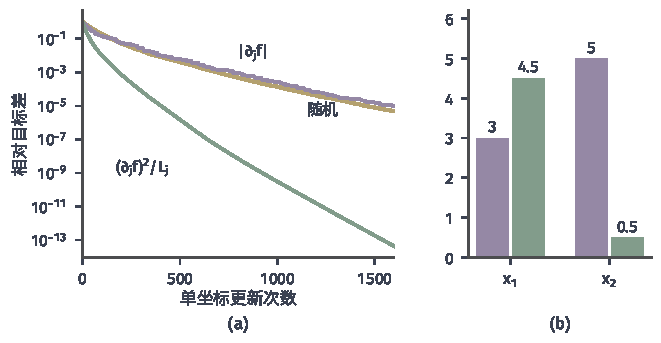
\includegraphics[width=112mm]{figures/05-optimization/04-block-optimization/matplotlib/block-greedy-rules/figure.pdf}
  \caption{选块指标的比较。(a)$N=80$、$n=40$的最小二乘，各列尺度相差很大，单坐标精确更新，纵轴为目标差与初值之比。黄线是均匀随机（$10$次重复的几何平均），紫线按$\lvert\partial_jf\rvert$选坐标，绿线按$(\partial_jf)^2/L_j$选坐标。(b)文中手算例子的两个坐标：紫色柱是$\lvert\partial_jf\rvert$，绿色柱是保底下降量$(\partial_jf)^2/(2L_j)$。}
  \label{fig:block-greedy-rules}
\end{BookInlineFigure}

图~\ref{fig:block-greedy-rules}(a)显示，当各列尺度差别很大时，只看偏梯度大小的规则并不比随机规则好，把曲率算进去之后才快了很多。(b)是手算的例子：两个指标选中了不同的坐标，而绿色柱才是能保证的下降量。

\paragraph{贪心指标的代价}
贪心规则需要知道所有块的偏梯度。若每次更新后要重算全部偏梯度，一步的代价就和一次全梯度相同，这时贪心规则很难划算。

当目标的耦合稀疏时，更新一块只影响少数几块的偏梯度，可以增量维护，并用优先队列取最大值，贪心规则才真正便宜。

\paragraph{复合目标的指标}
目标含非光滑项时，只看偏梯度会选错块。设$F=f+g$，$g(\bm{x})=\sum_Jg_J(\bm{x}_J)$是按块可分的凸函数，块$J$的二次上界加上$g_J$就成了局部模型。把模型能带来的下降量当作指标：
\begin{equation}
 \begin{aligned}
 \Delta_J^{g}(\bm{x})=-\min_{\bm{h}}\Bigl\{&\langle\nabla_Jf(\bm{x}),\bm{h}\rangle+\frac{L_J}{2}\lVert\bm{h}\rVert_2^2\\
 &+g_J(\bm{x}_J+\bm{h})-g_J(\bm{x}_J)\Bigr\}.
 \end{aligned}
 \label{eq:block-composite-index}
\end{equation}
取$g_J=\lvert\cdot\rvert$，当前$x_j=0$，$L_j=1$。若偏导数是$0.5$，$h=0$是最小点，指标为$0$，这个坐标不会动，尽管偏导数不为零。若偏导数是$2$，模型最小点是$h=-1$，指标为$0.5$，这一块才有进展可言。
